\section{Top Gear}

\begin{figure}[htbp]
\begin{center}
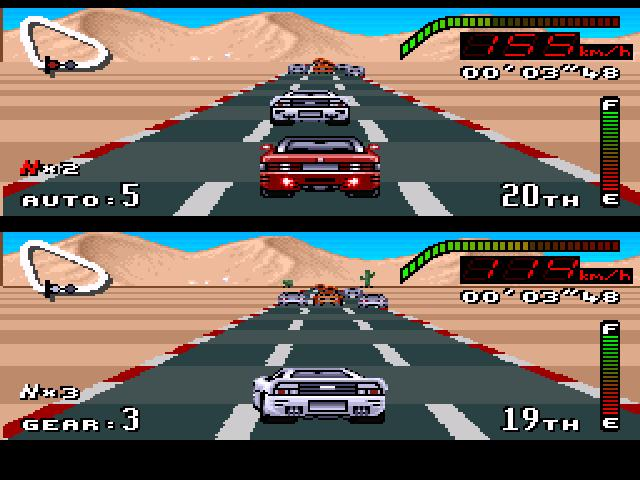
\includegraphics[width=.60\textwidth]{./imagenes/top_gear.jpg}
\caption{Top Gear}
\label{Top Gear}
\end{center}
\end{figure}
Top Gear\footnote{\url{http://es.wikipedia.org/wiki/Top_Gear_(videojuego)}} es un videojuego de carreras para Super Nintendo publicado en el año 1992. En el juego tienes que competir con 20 automóviles para llegar en el primer lugar y avanzar hacia el siguiente torneo. El modo de juego es sencillo, tan solo debes debes indicar mediante teclas la direción a la cual deseas que se dirija el auto.

\subsubsection{¿Por qué es uno de mis juegos favoritos?}
\begin{itemize}
	\item[Saulo Ronquillo]No es un juego muy complejo ni goza de gráficas espectaculares pero hasta el día de hoy me sigue entreteniendo mucho, durante el transcurso del juego las competencias se realizan en diferentes lugares del mundo lo cual ayuda a que el juego no sea monótomo y agregado a todo eso, la música\footnote{\url{http://archive.org/details/TopGearMusicaSnes}} del videojuego es muy, muy buena.
\end{itemize}
